\documentclass[../sparc.tex]{subfiles}
\graphicspath{{\subfix{../images/}}}
\begin{document}

%%%%%%%%%%%%%%%%%%%%%%%%%%%%%%%%%%%%%%%%%%%%%%%%%%%%%%%%%%%%%%%%%%%%%%%%%%%%%%%%
\section{Последовательный порт}
\label{section:communication-serial-port}
\index{Электроника!Последовательный порт}

%%%%%%%%%%%%%%%%%%%%%%%%%%%%%%%%%%%%%%%%%%%%%%%%%%%%%%%%%%%%%%%%%%%%%%%%%%%%%%%%
\subsection{Общие сведения}

\emph{Последовательный порт}, или по-английски ``serial port'' -- это один из
простейших способов коммуникации между цифровыми устройствами.

Как следует из названия, последовательный порт передаёт биты последовательно, по
одному за единицу времени.  Существуют другие аппаратные интерфейсы, которые
также используют последовательную передачу данных -- например, USB и Ethernet.
Однако последовательным портом обычно называется аппаратное обеспечение,
совместимое со стандартом RS-232 или подобными стандартами (например, RS-485,
RS-422.)

Последовательные порты разделяют на \emph{синхронные} (использующие специальный
тактирующий импульс для синхронизации приёмопередачи на устройствах) и
\emph{асинхронные} (где взаимодействующие устройства должны быть до начала
обмена данными быть настроены на одну и ту же скорость приёмопередачи.)

Последовательный порт как правило является \emph{полнодуплексным} средством
коммуникации, так как позволяет передавать данные в обе стороны.  Для этого
используются две независимые линии: одна -- для передачи данных (``Transmit'',
или ``Tx'') и другая -- для приёма (``Receive'', ``Rx''.)

\note{ Может возникнуть вопрос, почему обычно ``Receive'' сокращается до ``Rx'',
  а ``Transmit'' до ``Tx''.  Причину этому можно найти в истории: во времена
  использования телеграфа, отправка символа точки требовало больше усилий, чем
  отправка обычной буквы, из-за этого операторы использовали букву ``x'' вместо
  точки.

  Поскольку стоимость телеграфа была фиксированной: стоимость работы оператора,
  стоимость работы принтера, стоимость самой телеграфной линии между станциями.
  Чем больше данных вы могли передать, тем больше денег вы могли заработать.
  Это привело к появлению большого количества сокращений для часто используемых
  слов, особенно для длинных.  Таким образом, вместо длиного слова
  ``Transmission'' операторы телеграфа предпочитали писать просто ``T.'' (зная,
  что на другом конце их поймут.)  Однако символ точки не был доступен в
  телеграфе, когда использовался режим ввода букв.  Из-за этого операторам
  приходилось вводить символ ``T'', потом переключаться в режим ввода чисел (для
  ввода точки) и потом обратно переключаться в текстовый режим.  Это занимало
  много времени.  Поэтому, каждый раз, когда требовалось ввести символ точки,
  телеграфисты вместо него использовали сивол ``X'', который можно было ввести,
  не переключаясь в режим ввода чисел.  Поскльку очень мало английских слов
  заканчиваются на ``X'', то данный символ оказался идеальной заменой точки.

  Отсюда и пошли некоторые сокращения вроде ``Rx'' и
  ``Tx''.\autocite{so:krisw}
}

Недостатком последовательного порта является более низкая скорость передачи
данных по сравнению с \emph{параллельным портом}, где сразу можно передать 8
бит.  Однако для единовременной передачи 8 бит параллельному порту требуется 8
проводов между передачиком и приёмником, тогда как для последовательного порта
нужно всего два провода для передачи данных.  Таким образом, последовательная
передача данных является более компактной.

%%%%%%%%%%%%%%%%%%%%%%%%%%%%%%%%%%%%%%%%%%%%%%%%%%%%%%%%%%%%%%%%%%%%%%%%%%%%%%%%
\subsection{Универсальный асинхронный приёмопередатчик (UART)}
\label{section:communication-uart}

Универсальный асинхронный приёмопередатчик, более широко известный под
англоязычным названием \gls{UART} (англ. \emph{Universal Asynchronous
Receiver-Transmitter}) -- это специальное устройство или логическая цепь для
асинхронной последовательной передачи данных.  По сути UART является одной из
реализаций последовательного порта, которая широко используется для обмена
данными между устройствами.

Для осуществления передачи UART получает данные и последовательно пересылает их
в виде отдельных бит по шине, отправляя их через равные промежутки времени.  На
приёмнике второй UART собирает полученные биты в исходные байты.  И на
передатчике, и на приёмнике имеется специальная микросхема, называемая
\emph{сдвиговый регистр}, которая являеется фундаментальным способом
преобразования между последовательным и параллельным представлением данных.

Пример передачи 1 байта информации визуализирован в виде диаграммы на рисунке
\ref{fig:communication-serial-port-diagram}.  Данная диаграмма показывает
изменение напряжения во времени на линии Rx-Tx между двумя условными
устройствами.

\begin{figure}[ht]
  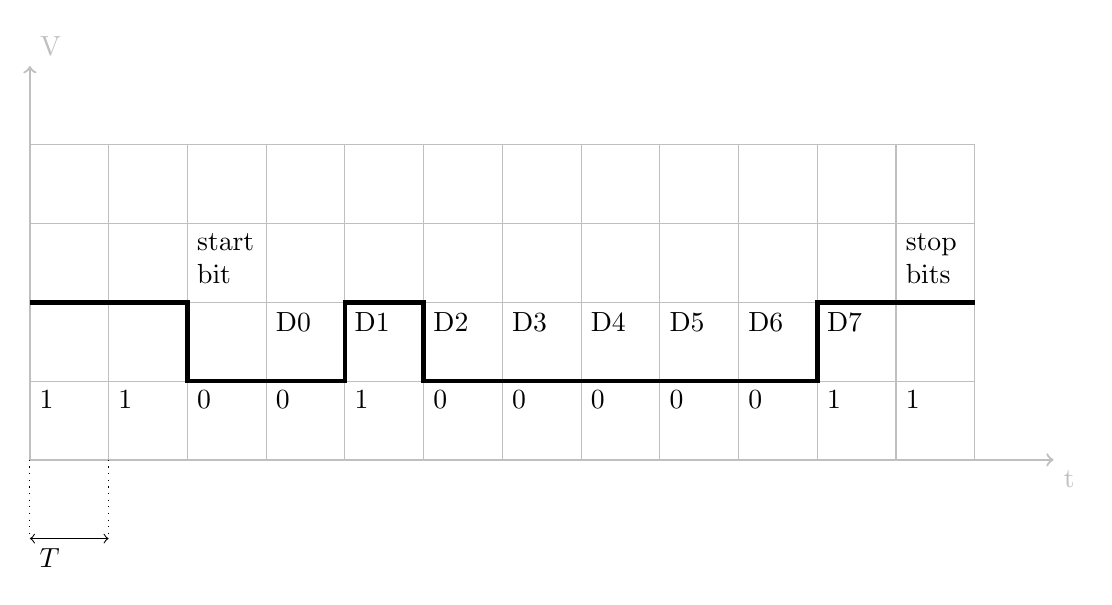
\begin{tikzpicture}
    \draw[lightgray] (0, 0) grid (12, 4);
    \draw[lightgray, thick, ->] (0, 0) -- (13, 0) node[anchor=north west] {t};
    \draw[lightgray, thick, ->] (0, 0) -- (0,  5) node[anchor=south west] {V};
    \draw[ultra thick, black] (0,  2) -- (2,   2)
    %% 0 (start bit)
    -- (2,   1) -- (3,   1)
    %% 0
    -- (4,   1)
    %% 1
    -- (4,   2) -- (5,   2)
    %% 0 x 5
    -- (5,   1) -- (10,   1)
    %% 1
    -- (10,   2)
    -- (11,   2)
    %% 1 (stop bits)
    -- (12,   2);
    %% Draw digits.
    \draw[black]
    (0,  1) node[anchor=north west] {1}
    (1,  1) node[anchor=north west] {1}
    (2,  1) node[anchor=north west] {0}
    (3,  1) node[anchor=north west] {0}
    (4,  1) node[anchor=north west] {1}
    (5,  1) node[anchor=north west] {0}
    (6,  1) node[anchor=north west] {0}
    (7,  1) node[anchor=north west] {0}
    (8,  1) node[anchor=north west] {0}
    (9,  1) node[anchor=north west] {0}
    (10, 1) node[anchor=north west] {1}
    (11, 1) node[anchor=north west] {1};
    %% Draw comments.
    \draw[black]
    (2,  3) node[anchor=north west, text width=1cm] {start bit}
    (11, 3) node[anchor=north west, text width=1cm] {stop bits};
    %% Draw bits.
    \draw[black]
    (3,  2) node[anchor=north west] {D0}
    (4,  2) node[anchor=north west] {D1}
    (5,  2) node[anchor=north west] {D2}
    (6,  2) node[anchor=north west] {D3}
    (7,  2) node[anchor=north west] {D4}
    (8,  2) node[anchor=north west] {D5}
    (9,  2) node[anchor=north west] {D6}
    (10, 2) node[anchor=north west] {D7};
    \draw[black, dotted] (0, 0) -- (0, -1);
    \draw[black, dotted] (1, 0) -- (1, -1);
    \draw[<->, black]
    (0, -1) node[anchor=north west, text width=1cm] {$T$}
    -- (1, -1);
  \end{tikzpicture}
  \caption{Передача символа 'A' (код 65 в таблице ASCII, соответствет двоичному
    коду \texttt{01000001}) по последовательному порту.}
  \label{fig:communication-serial-port-diagram}
\end{figure}

Скорость пересылки данных определяется параметром, называемым битрейт
(англ. \emph{bit rate}) или бодрейт (англ. \emph{baud rate}), который измеряется
в бодах (битах в секунду.)  Скорость $S$ (в бодах) и длительность одного бита
$T$ (в секундах) связаны отношением \ref{equation:uart-speed}.

\begin{equation}
  T = \frac{1}{S}
  \label{equation:uart-speed}
\end{equation}

Где $T$ определяет длительность одного бита и зависит от скорости передачи
данных (см. рисунок \ref{fig:communication-serial-port-diagram}.)

Общепринятными скоростями считаются: 300, 1200, 2400, 4800, 9600, 19200, 38400,
57600, 115200, 230400, 460800 и 921600 бод.

Если подставить в формулу \ref{equation:uart-speed} скорость 9600 бод, то получаем:

\begin{equation}
  T = \frac{1}{9600} \approx 0.00010416 \mbox{с} \approx 104.16 \mbox{мкс}
\end{equation}

Таким образом, для 9600 бод время пересылки одного бита составляет примерно
104.16 мкс.  Для сравнения, минимальное время одного мигания глазами у человека
составляет $\approx100 \mbox{мс}$\cite{chudler}, что в $\approx960$ медленнее,
чем пересылка одного бита для такой скорости.

Обратите внимание, что для успешной коммуникации у приёмника и передатчика
должны быть одинаковые скорости последовательного порта, в противном случае
данные будут читаться не верно.  Это связано с тем, что приёмник и передатчик не
имеют тактирующего сигнала, синхронизирующего пересылку данных.

Иногда бывает удобнее оперировать не битами в секунду, а байтами в секунду,
поскольку в большинстве случаев мы измеряем объём информации именно в байтах.
Чтобы пересчитать боды в байты в секуду, необходимо использовать формулу
\ref{equation:uart-bauds-to-bytes-per-sec} (предполагается, что в 1 байте 8
бит.)

\begin{equation}
  S_{\mbox{байты/с}} = \frac{S_{\mbox{биты/с}}}{8}
  \label{equation:uart-bauds-to-bytes-per-sec}
\end{equation}

\example{ Популярной скоростью передачи текстовых данных при использовании
  Arduino является 9600 бод.  По формуле
  \ref{equation:uart-bauds-to-bytes-per-sec} мы можем узнать, сколько байт за
  секунду можно передать между компьютером и Arduino:
  \begin{equation}
    S_{\mbox{байты/с}} = \frac{9600_{\mbox{биты/с}}}{8} = 1200 \mbox{байт/с} = 1.2 \mbox{КБ/с}
  \end{equation}

  Допустим, в среднем размер одной музыкальной композиции составляет 5 МБ.  Если
  мы заходим передать музыкальную композицию с компьютера на Arduino со
  скоростью 9600 бод, то мы можем посчитать, сколько времени на это потребуется:
  \begin{align*}
    5 \mbox{МБ} = 5242880 \mbox{байт}\\
    T = \frac{5242880 \mbox{байт}}{1200 байт} \approx 4369,06 \mbox{с} \approx 72.8 \mbox{мин.}
  \end{align*}

  Таким образом получаем, что для передачи 5 МБ данных потребуется 72 минуты
  времени, то есть, больше часа.
}

%%%%%%%%%%%%%%%%%%%%%%%%%%%%%%%%%%%%%%%%%%%%%%%%%%%%%%%%%%%%%%%%%%%%%%%%%%%%%%%%
\subsection{Работа с аппаратным последовательным портом}

\subsubsection{Класс \texttt{Serial}}

В Arduino для работы с последовательным портом есть класс \texttt{Serial},
который позволяет настраивать параметры передачи данных через последовательный
порт, передавать и принимать данные.  Мы уже работали с последовательным портом
в главе \ref{section:serial-port}, сейчас мы посмотрим на него более пристально.

На всех платах Arduino есть как минимум один последовательный порт, на некоторых
моделях (вроде Arduino Mega 2560) есть несколько последовательных портов.
Таблица последовательных портов и ассоциированных с ними цифровых портов можно
найти в таблице \ref{table:serial-ports--pins} (данные взяты из описания
\texttt{Serial} в \cite{arduino:reference}.)

\begin{table}[h]
\centering
\begin{tabular}{|m{9em}|m{3.5em}|m{3.5em}|m{3.5em}|m{3.5em}|m{3.5em}|}
  \hline
  \multirow{2}{2em}{\textbf{Плата}} & \multicolumn{5}{c|}{\textbf{Цифровые порты}} \\
  \cline{2-6}
   & \textbf{Serial}  & \textbf{Serial1}     & \textbf{Serial2}     & \textbf{Serial3}     & \textbf{Serial4}     \\
\hline
UNO R3, UNO R3 SMD Mini    & 0(RX), 1(TX) &                  &                  &                  &                  \\
\hline
Nano (classic)             & 0(RX), 1(TX) &                  &                  &                  &                  \\
\hline
UNO R4 Minima, UNO R4 WiFi &              & 0(RX0), 1(TX0)   &                  &                  &                  \\
\hline
Leonardo, Micro, Yún Rev2  &              & 0(RX), 1(TX)     &                  &                  &                  \\
\hline
Uno WiFi Rev.2             &              & 0(RX), 1(TX)     &                  &                  &                  \\
\hline
MKR boards                 &              & 13(RX), 14(TX)   &                  &                  &                  \\
\hline
Zero                       &              & 0(RX), 1(TX)     &                  &                  &                  \\
\hline
GIGA R1 WiFi               &              & 0(RX), 1(TX)     & 19(RX1), 18(TX1) & 17(RX2), 16(TX2) & 15(RX3), 14(TX3) \\
\hline
Due                        & 0(RX), 1(TX) & 19(RX1), 18(TX1) & 17(RX2), 16(TX2) & 15(RX3), 14(TX3) &                  \\
\hline
Mega 2560 Rev3             & 0(RX), 1(TX) & 19(RX1), 18(TX1) & 17(RX2), 16(TX2) & 15(RX3), 14(TX3) &                  \\
\hline
Nano 33 IoT                &              & 0(RX0), 1(TX0)   &                  &                  &                  \\
\hline
Nano RP2040 Connect        &              & 0(RX0), 1(TX0)   &                  &                  &                  \\
\hline
Nano BLE / BLE Sense       &              & 0(RX0), 1(TX0)   &                  &                  & \\
\hline
\end{tabular}
\caption{Последовательные порты на Arduino.}
\label{table:serial-ports--pins}
\end{table}

У каждого последовательного порта есть ассоциированные с ним цифровые порты
Arduino.  На большинстве плат Arduino для последовательного порта по-умолчанию
используются порты 0 (RX) и 1 (TX.)  При передачи данных между компьютером и
Arduino используется именно этот \texttt{Serial}; таким образом передаваемые
значения дублируются на цифровых портах, связанных с данным последовательном
портом.

\note{Обратите внимание, что если на Arduino цифровые порты, связанные с
  \texttt{Serial} (обычно это порты 0 и 1) зайдействовать, например, для мигания
  светодиодами, то это может помешать корректной загрузке программы в Arduino.
  В таком случае может потребоваться отключение внешних устройств от портов 0 и
  1 на время перепрошивки.  По этой причине лучше не использовать данные порты
  без необходимости.}

\subsubsection{Передача данных на компьютер}

Для того, чтобы передавать данные на компьютер, необходимо настроить скорость
передачи данных.  Это разумно производить внутри функции \texttt{setup}, так как
скорость обычно задаётся один раз и не меняется на протяжении всей работы с
последовательным портом.

Задание скорости передачи данных производится с помощью метода \texttt{begin} из
класса \texttt{Serial}.  В примере ниже мы задаём скорость, равную 9600 бод:

\begin{minted}{cpp}
  void setup() {
    Serial.begin(9600);
  }
\end{minted}

Далее мы можем передать данные на компьютер.  Для передачи данных в классе
\texttt{Serial} существуют методы \texttt{print} и \texttt{println}.  Метод
\texttt{println} в отличии от \texttt{print} отправляет данные в порт с
добавлением в конец данных символа перевода на новую строку.

Пример отправки строки на компьютер:

\begin{minted}{cpp}
  void loop() {
    Serial.println("Hello World");
  }
\end{minted}

Обратите внимание, что методы передачи данных позволяют работать с данными
разных типов, Так, например, с помощью \texttt{println} вы можете передать не
только строки, но и числа -- компьютер сам ``поймёт'', как правильно эти данные
подготовить к отправке:

\begin{minted}{cpp}
  void loop() {
    Serial.println(42);
  }
\end{minted}

Все данные перед передачей преобразуются в строку, которая затем отправляется
через последовательный порт.

\subsection{Приём данных с компьютера}

Класс \texttt{Serial} предоставляет ряд методов, которые предназначены для
чтения данных из последовательного порта.

Данные, которые приходят от компьютера, буферизируются на стороне Arduino.
Размер буфера составляет 64 байта (см. документацию на метод
\texttt{Serial.available} в \cite{arduino:reference}.)  Класс \texttt{Serial}
предоставляет метод метод \texttt{available}, который при вызове возвращает
количество байт, доступных в буфере для чтения.  Обычно данный метод
используется перед тем, как производится чтение данных.

Чтение данных осуществляется несколькими способами, в зависимости от типа
принимаемых данных.  Самым примитивным вариантом является чтение байт с помощью
метода \texttt{read}.  Каждый вызов \texttt{read} возвращает следующий доступный
байт из буфера приёма.  Когда данных в буфере нет, \texttt{read} возвращает
значение -1.

\note{ Обратите внимание, что \texttt{read} возвращает тип \texttt{int}, а не
  \texttt{byte} или \texttt{char}.  Это обусловлено тем, что если бы
  \texttt{read} возвращал \texttt{byte} (у которого нет отрицательной части), то
  он не мог бы вернуть значение -1, а без этого было бы невозмозжно
  сигнализировать о конце данных с помощью возвращаемого значения.  С другой
  стороны, если бы \texttt{read} возвращал \texttt{char}, то данная проблема
  решилась бы (у \texttt{char} диапазон от -128 до 127), однако при этом стало
  бы проблематично получать значения от 128 до 255 (максимальное значение,
  которое можно записать в 1 байт.)}

Пример чтения данных можно увидеть в следующем листинге:

\begin{minted}{cpp}
  void loop() {
    if (Serial.available() > 0) {
      int incoming_byte = Serial.read();
      // ... Обработка данных ...
    }
  }
\end{minted}

\subsection{Программная реализация последовательного порта}

Встроенная библиотека
\texttt{SoftwareSerial}\footnote{\url{https://docs.arduino.cc/learn/built-in-libraries/software-serial/}}
позволяет программно реализовать последовательный протокол на цифровых портах,
отличных от тех, что указаны в таблице \ref{table:serial-ports--pins}.

С помощью данной библиотеки можно реализовать несколько последовательных портов
со скоростями до 115200 бод.

Тем не менее, \texttt{SoftwareSerial} имеет ряд серьёзных ограничений:
\begin{itemize}
\item Библиотека позволет в каждый момент времени либо передавать, либо
  принимать данные -- одновременный приём и передача не возможны. Таким образом
  можно сказать, что коммуникация выполняется в \emph{полу-дуплексном режиме}.
\item Если используется несколько \texttt{SoftwareSerial}-портов, то только один
  из них может принимать данные в каждый момент времени.  Это связано с тем, что
  приём данных происходит по прерываниям.
\item Для приёма данных необходимо задействовать только те порты, которые
  поддерживают прерывания.
\item На платах Arduino и Genuino 101 максимальная скорость передачи данных
  составляет 57600 бод.
\item На платах Arduino и Genuino 101 порт номер 13 не может быть использован в
  роли RX-порта.
\end{itemize}

Пример создания программного последовательно порта показан ниже.

\begin{listing}[H]
  \begin{minted}{cpp}
    #include <SoftwareSerial.h>

    const byte RX_PIN = 2;
    const byte TX_PIN = 3;

    SoftwareSerial my_serial(RX_PIN, TX_PIN);

    void setup() {
      my_serial.begin(9600);
      my_serial.println("Hello, World!");
    }

    void loop() {

    }
  \end{minted}
  \label{listing:communication-serial-software}
  \caption{Пример использования программного последовательного порта
    (\texttt{SoftwareSerial}.)}
\end{listing}

Поскольку программная реализация последовательного порта основывается на
механизме прерываний, то при высоких скоростях приёма данных может возникнуть
``голод прерываний'' -- это значит, что микроконтроллер будет большую часть
времени проводить за обработкой приходящих данных, отдавая на остальные задачи
минимум времени.  В таком случае, например, функция \texttt{loop} практически не
будет получать процессорного времени (т.е. не будет вызываться), а также другие
прерывания (например, от кнопок) не смогут быть обработаны.

\subsection{Пример: Передача данных между двумя Arduino}

Теперь мы рассмотрим комплексный пример, в котором будет показана работа как с
аппаратным последовательным портом, так и с программной его версией.  Для этого
нам потребуется две Arduino, между которыми мы будем передавать данные.

Для передачи данных будем использовать \texttt{SoftwareSerial}, с портам 10 (RX)
и 11 (TX).  Первая Arduino будет передавать через последовательный порт на
вторую Arduino поочерёдно символ \texttt{'1'} и \texttt{'0'}.  Вторая Arduino
будет при получении \texttt{'1'} включать светодиод на 13-м порту, и при
получении \texttt{'0'} выключать его.

Порт 11 (TX) на Arduino-передатчике следует соединить с портом 10 (RX) на
Arduino-приёмнике.  Также следует соединить \texttt{GND} двух Arduino вместе,
чтобы у них был одинаковый логический уровень нуля.  На
рис. \ref{fig:arduino-serial-communication-1} показан пример, как можно
соединить две Arduino Mega 2560 для данного проекта.  Можно использовать другие
модели Arduino, адаптировав соответствующим образом подключение и код.

\begin{figure}[H]
  \centering
  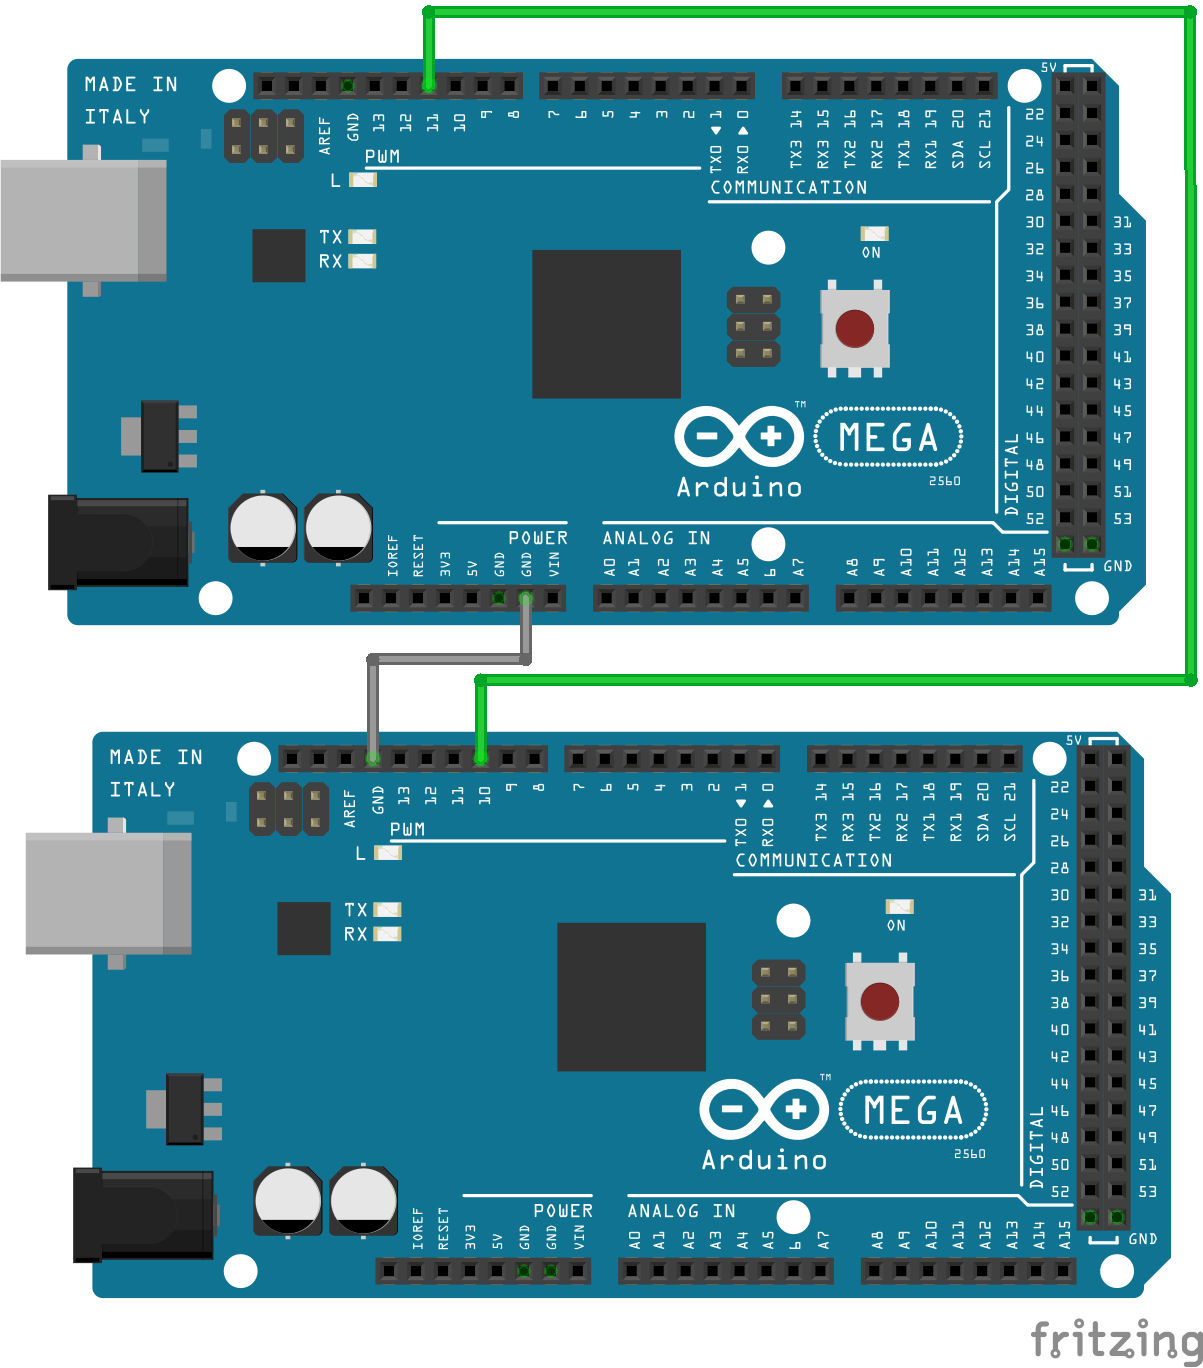
\includegraphics[width=10cm]{schematics/arduino-serial-communication-1}
  \caption{Соединение двух Arduino Mega 2560 через UART в режиме симплексной
    (односторонней) передачи.  Верхняя Arduino является передатчиком, нижняя --
    приёмником.}
  \label{fig:arduino-serial-communication-1}
\end{figure}

Программный код будет один и тот же для обоих Arduino, переключение в режим
приёмника производится через замыкание порта 4 на \texttt{GND}; если же порт не
замкнут, то Arduino работает в режиме передатчика.  Полностью код можно увидеть
в листинге \ref{listing:communication-serial-two-arduino-example}.

Обратите внимание, что вместо провода, соединяющего RX-TX двух Arduino можно
использовать более изощрённый способ связи: лазер.  Если подключить модуль
лазера (вроде того, что показан на рис. \ref{fig:arduino-laser-module}) к TX
первой Arduino и направить лучше лазера на фоторезистор, подключенный на порт RX
второй Arduino, то можно переправлять данные по лазерному лучу.  В таком случае
мы можем наглядно видеть, как организована последовательная передача данных: при
передаче единицы лазер горит, при передаче нуля -- гаснет.

\begin{figure}[ht]
  \centering
  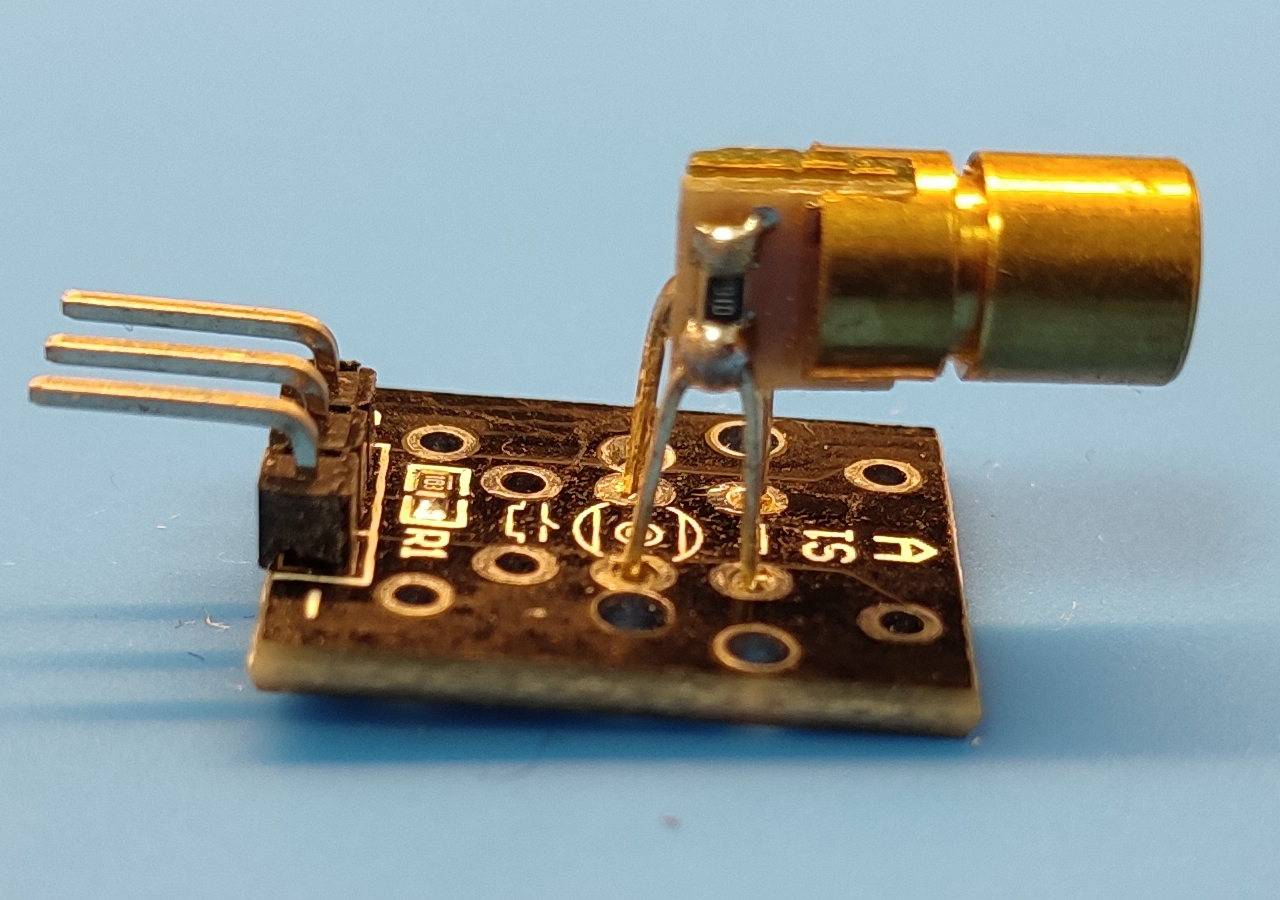
\includegraphics[width=10cm]{arduino-laser-module}
  \caption{Модуль лазера для Arduino.}
  \label{fig:arduino-laser-module}
\end{figure}


Самая большая сложность при использовании лазера -- это настроить
светочувствительный датчик так, чтобы Arduino различала нули и единицы.  Проще
всего этого добиться, собрав делитель напряжения, где одно ``плечо'' делителя
будет нашим фоторезистором (назовём его $R_1$), а другое ``плечо'' --
потенциометром (назовём его $R_2$.)  Это позволит регулировать отношение $R_1$ и
$R_2$, меняя таким образом уровень напряжения, которое будет получать Arduino
при изменении сопротивления $R_1$.  Путём ручной настройки можно добиться, чтобы
при отсутствии света лазера фоторезистор выдавал уровень напряжения,
соответсвующий логическому нулю на цифровой порт, а при подаче света лазера --
уровень, соответствующий логической единице.

\begin{listing}[H]
  \begin{minted}{cpp}
    #include <SoftwareSerial.h>
    const byte RX_PIN = 10;
    const byte TX_PIN = 11;
    SoftwareSerial software_serial(RX_PIN, TX_PIN);

    const byte SWITCH_PIN = 4;
    const byte LED_PIN = 13;

    void setup() {
      pinMode(SWITCH_PIN, INPUT_PULLUP);
      pinMode(LED_PIN, OUTPUT);
      Serial.begin(9600);
      software_serial.begin(600);
    }

    void transmit() {
      software_serial.print(1);
      delay(1000);
      software_serial.print(0);
      delay(1000);
    }

    void receive() {
      if (software_serial.available() > 0) {
        byte value = software_serial.read();
        Serial.print("VALUE: ");
        Serial.println(value);
        if (value == '1') {
          digitalWrite(LED_PIN, HIGH);
          Serial.println("ON");
          delay(1000);
        } else if (value == '0') {
          digitalWrite(LED_PIN, LOW);
          Serial.println("OFF");
          delay(1000);
        }
      }
    }

    void loop() {
      if (digitalRead(SWITCH_PIN) == HIGH) {
        transmit();
      } else {
        receive();
      }
    }
  \end{minted}
  \label{listing:communication-serial-two-arduino-example}
  \caption{Пример симплексной (однонаправленной) связи двух Arduino через
    программный последовательный порт.}
\end{listing}


\end{document}
